\chapter{Laboratorio 2}
\section{Introduzione}
Nell'esperienza di laboratorio precedente, si è realizzato un circuito a guadagno unitario, che realizza una funzione di buffer replicando il segnale in ingresso sull'uscita. Inoltre, esso ha anche una funzione di disaccoppiamento tra ingresso e uscita, con una resistenza di ingresso tendente ad infinito e una resistenza di uscita tendente a zero. 

In questa esperienza di laboratorio, si sono inizialmente effettuate ulteriori misure sul circuito \textit{emitter follower} per poi realizzare una versione \textit{single-ended} dell'\textit{emitter follower}.

\section{Grafico ingresso-uscita \textit{emitter follower}}
Di seguito vengono riportati i risultati delle misure effettuate sul circuito precedentemente realizzato. In ingresso al circuito è stato applicato un segnale sinusoidale con frequenza pari a \SI{1}{\kilo\hertz} e tensione picco-picco variabile da \SI{0.5}{\volt} a \SI{5}{\volt} con step di \SI{0.5}{\volt}. Sono state poi misurate le tensioni picco-picco in ingresso Vpp\sub{i} e in sucita Vpp\sub{o} al circuito grazie alle funzioni integrate dell'oscilloscopio. Per rendere stabile il valore della misura ricavata dall'oscilloscopio, è stato selezionato un filtro a \SI{20}{\mega\hertz} sugli ingressi dell'oscilloscopio e sono state effettuate delle medie (di 6
 campioni) sui segnali. In questo modo è stato possibile ottenere un segnale più pulito da disturbi e rumore (\Fig\ref{fig:emitterfollwer_misurepiccopicco}).
\begin{table}[h!]
	\centering
	\begin{tabular}{c|c}
		\hline
		Vpp\sub{i} [V] & Vpp\sub{o} [V]\\ \hline
		0.509 & 0.491 \\ \hline
		1.019 & 0.984 \\ \hline
		1.502 & 1.476 \\ \hline
		2.080 & 1.994 \\ \hline
		2.565 & 2.474 \\ \hline
		3.037 & 2.962 \\ \hline
		3.524 & 3.459 \\ \hline
		4.022 & 3.967 \\ \hline
		4.606 & 4.470 \\ \hline
		5.089 & 4.945 \\ \hline
	\end{tabular}
\end{table}
\begin{figure}[h!]
	\centering
	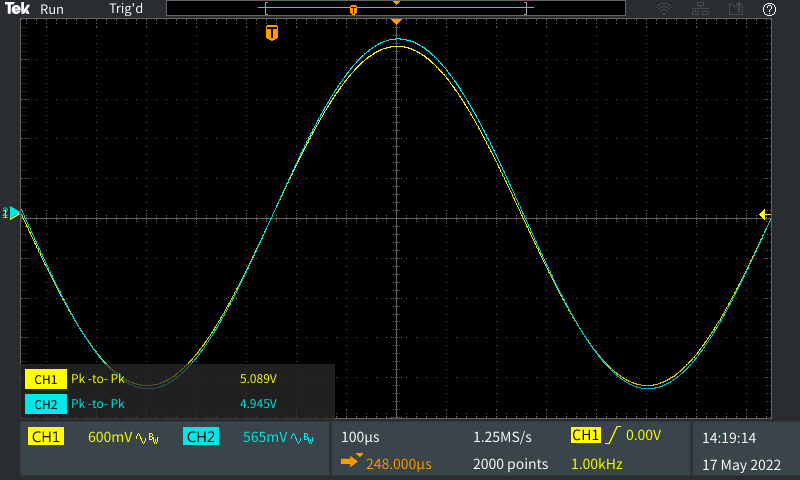
\includegraphics[width=0.7\linewidth]{./ImageFiles/Laboratorio 2/TEK00012}
	\caption{Misurazione della tensione picco-picco del segnale in ingresso (CH1) e in uscita (CH2) con i relativi valori picco-picco misurati dall'oscilloscopio.}
	\label{fig:emitterfollwer_misurepiccopicco}
\end{figure}
\todo{c'è un pezzo su modello equivalente del circuito  non so cosa è}
Come si può notare dalla tabella, il valore del guadagno del circuito è leggermente inferiore a uno. Cerchiamo di quantificare in modo quantitativo quanto il guadagno effettivo del circuito si discosta dal valore teorico unitario. Per fare ciò, rappresentiamo su un grafico il valore picco-picco di tensione misurato all'uscita del circuito in funzione della tensione in ingresso (valori riportati nella tabella precedente). Successivamente, eseguiamo un'interpolazione lineare della retta $y=a+bx$ che approssimi i valori ottenuti. Idealmente, vorremmo ottenere $a=1$ e $b=0$. Infatti, il coefficiente angolare della retta rappresenta il guadagno del circuito, mentre l'intercetta un eventuale offset.

Nella figura \ref{fig:emitterfollwer_inout} viene mostrato il risultato della retta interpolata sui dati stimata grazie alla funzione \textit{fitlm} offerta da Matlab. La retta identificata è $Vpp_o=-0.009+0.977*Vpp_i$. Come si poteva già intuire dalla tabella, abbiamo un guadagno leggermente inferiore a uno ma con un valore molto prossimo.
\begin{figure}[h!]
	\centering
	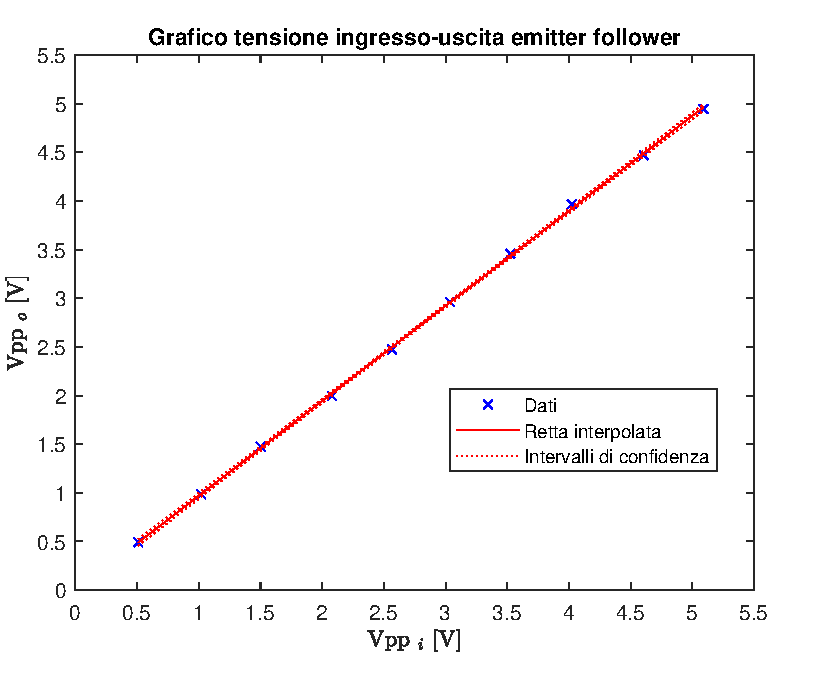
\includegraphics[width=0.7\linewidth]{./OtherFiles/Laboratorio 2/emitter follower-ingresso_uscita}
	\caption{Grafico ingresso-uscita del circuito emitter-follower.}
	\label{fig:emitterfollwer_inout}
\end{figure}

\section{Emitter follower single-ended: prima versione}
Si vuole ora modificare il circuito precedente in modo da alimentarlo tra alimentazione positiva e massa, senza la necessità di utilizzare una alimentazione negativa, realizzando il seguente circuito:
\begin{figure}[h!]
	\centering
	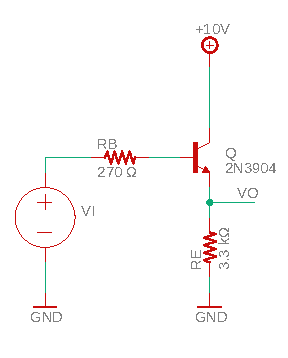
\includegraphics[width=0.4\linewidth]{./OtherFiles/Laboratorio 2/emitter follower}
	\caption{Schematico della prima versione del circuito emitter follower single-ended.}
	\label{fig:emitterfollwer_se}
\end{figure}
Tuttavia, alimentando questo circuito e applicando una tensione in ingresso V\sub{i} con frequenza di \SI{1}{\kilo\hertz} e tensione picco-picco di \SI{4}{\volt}, il circuito non funziona. Analizziamo il punto di lavoro stazionario (\Fig\ref{fig:emitterfollwer_se_DC}).
\begin{figure}[h!]
	\centering
	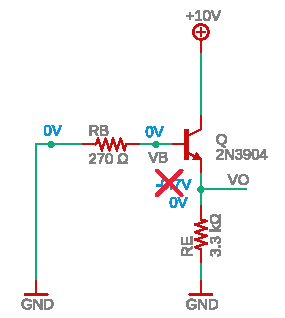
\includegraphics[width=0.4\linewidth]{./OtherFiles/Laboratorio 2/emitter follower_punto di lavoro-printout}
	\caption{Analisi punto di lavoro del circuito emitter follower single-ended.}
	\label{fig:emitterfollwer_se_DC}
\end{figure}
Supponiamo che il transistor sia in zona attiva diretta e con $\beta\to\infty$, con corrente di base nulla. Allora la tensione al nodo V\sub{B} è di \SI{0}{\volt}, poiché non c'è caduta di potenziale in una resistenza attraversata da corrente nulla. Dalle ipotesi fatte, se ne deduce che la tensione al nodo V\sub{o} dovrebbe essere pari a \SI{-0.7}{\volt} (caduta di tensione giunzione base-emettitore). Tuttavia, se così fosse, nella resistenza R\sub{E} scorrerebbe una corrente da massa verso V\sub{o}, in quanto ci sarebbe una differenza di potenziale ai capi della resistenza. Questo però non è possibile: infatti, la corrente dovrebbe poi entrare nel transistor dall'emettitore. Per costruzione, non è però possibile avere una corrente entrante nell'emettitore di un transistor bipolare. Per questo motivo, l'unica soluzione ammissibile è che la corrente che attraversa la resistenza sia nulla e che il circuito sia spento: il nodo V\sub{o} di trova a una tensione di \SI{0}{\volt}. 

Tuttavia, quando applichiamo un segnale alla base con ampiezza maggiore di \SI{0.7}{\volt}, il circuito si accende (\Fig\ref{fig:emitterfollwer_se_statocircuito}). Infatti, il nodo V\sub{o} si porta a una tensione maggiore di \SI{0}{\volt} e il transistor è polarizzato correttamente.
\begin{figure}[h!]
	\centering
	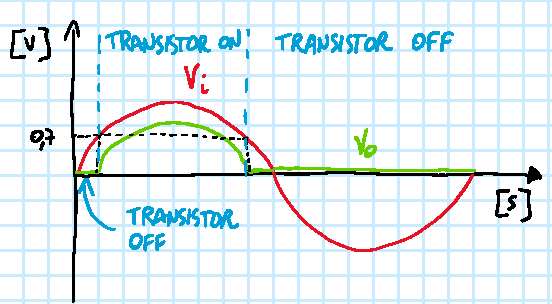
\includegraphics[width=0.7\linewidth]{./ImageFiles/Laboratorio 2/emitter follower errore soglia}
	\caption{Rappresentazione dello stato del circuito in funzione della tensione in ingresso.}
	\label{fig:emitterfollwer_se_statocircuito}
\end{figure}

Questo comportamento è stato verificato sul circuito reale. In figura \ref{fig:emitterfollwer_se_errore} si riportano le misure effettuate.
\begin{figure}[h!]
	\centering
	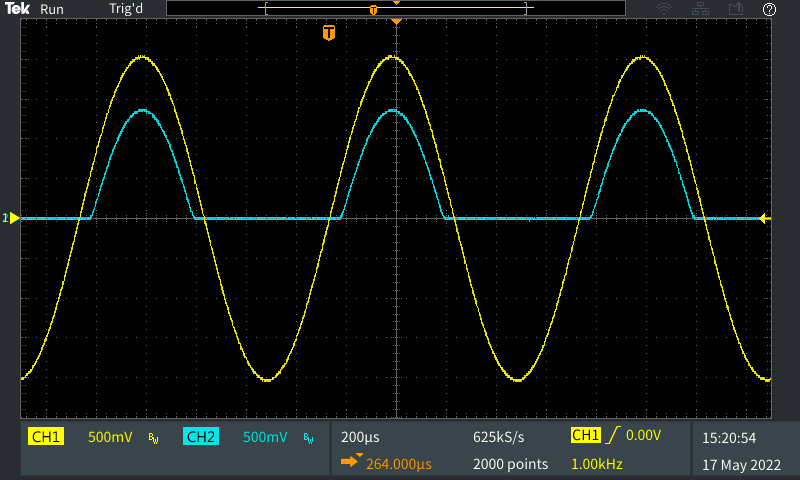
\includegraphics[width=0.7\linewidth]{./ImageFiles/Laboratorio 2/TEK00020}
	\caption{Misurazione della tensione in ingresso (CH1) e in uscita (CH2) del circuito emitter follower single-ended analizzato precedentemente con tensione picco-picco di \SI{4}{\volt} e frequenza \SI{1}{\kilo\hertz}.}
	\label{fig:emitterfollwer_se_errore}
\end{figure}

Per far funzionare correttamente il circuito bisognerebbe alzare la tensione di base, aggiungendo un offset nel segnale, in modo che il transistor sia sempre polarizzato correttamente lungo tutto il periodo della sinusoide.

\section{Emitter follower single-ended: seconda versione}
Per garantire la corretta polarizzazione del transistor, applicando una tensione di offset sulla base, è stato inserito un partitore di tensione realizzato con le resistenze R\sub{1} e R\sub{2}, rispettivamente di valore \SI{130}{\kilo\ohm} e \SI{150}{\kilo\ohm} (\Fig\ref{fig:emitterfollwer_v2}). In questo modo, supponendo la corrente di base nulla (ossia $\beta\to\infty$) la tensione V\sub{B} si ottiene:
\begin{equation}
	V_B= \SI{10}{\volt}*\frac{R_2}{R_2+R_1}
	=\SI{10}{\volt}*\frac{\SI{150}{\kilo\ohm}}{\SI{150}{\kilo\ohm}+\SI{130}{\kilo\ohm}}\simeq\SI{5.357}{\volt}
	\label{eq:1}
\end{equation}
\begin{figure}[h!]
	\centering
	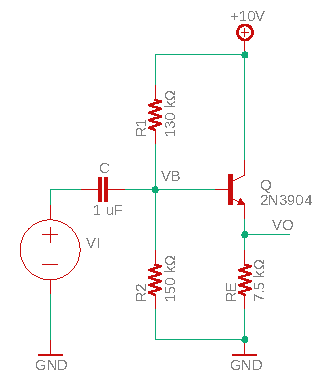
\includegraphics[width=0.4\linewidth]{./OtherFiles/Laboratorio 2/emitter follower_v2}
	\caption{Schematico della seconda versione del circuito emitter follower single-ended.}
	\label{fig:emitterfollwer_v2}
\end{figure}

Si noti come è stato necessario inserire un condensatore \textit{C} tra V\sub{i} e V\sub{B} in modo da disaccoppiare in continua i due nodi. Se non si inserisse un condensatore, il generatore V\sub{i} porterebbe la tensione al nodo V\sub{B} a massa nell'analisi del punto di lavoro, riportando il circuito nella situazione precedente.

\subsection{Componenti e misure}
Per realizzare il circuito in laboratorio (\Fig\ref{fig:emitterfollwer_v2_circuito}), si sono utilizzati i seguenti componenti:
\begin{itemize}
	\item transistor 2N3904;
	\item tre resistenze rispettivamente da R\sub{11}=\SI{12}{\kilo\ohm}, R\sub{12}=\SI{39}{\kilo\ohm} e R\sub{13}=\SI{82}{\kilo\ohm} connesse in serie per realizzare la resistenza R\sub{1};
	\item tre resistenze rispettivamente da R\sub{21}=\SI{39}{\kilo\ohm}, R\sub{22}=\SI{39}{\kilo\ohm} e R\sub{23}=\SI{82}{\kilo\ohm} connesse in serie per realizzare la resistenza R\sub{2};
	\item due resistenze rispettivamente da R\sub{E1}=\SI{3.9}{\kilo\ohm}, R\sub{E2}=\SI{3.9}{\kilo\ohm} connesse in serie per realizzare la resistenza R\sub{E};
	\item condensatore C da \SI{1}{\micro\farad}.
\end{itemize}

\begin{figure}[h!]
	\centering
	\includegraphics[width=0.7\linewidth,angle=-90]{./ImageFiles/Laboratorio 2/IMG\_20220517\_122529}
	\caption{Foto del circuito realizzato in laboratorio. `E possibile notare anche i terminali per l'applicazione del segnale a un capo del condensatore.}
	\label{fig:emitterfollwer_v2_circuito}
\end{figure}

Inoltre, sono state utilizzate i seguenti strumenti:
\begin{itemize}
	\item alimentatore da banco con tensione positiva \SI{10}{\volt} e limite in corrente di \SI{50}{\milli\ampere};
	\item oscilloscopio a due canali;
	\item generatore di forme d'onda;
	\item multimetro da banco.
\end{itemize}

I valori significativi di tutti i componenti sono stati misurati attraverso il multimetro. Di seguito si riportano le misure effettuate:
\begin{table}[h!]
	\centering
	\begin{tabular}{c|c|c}
		\hline
		Componente & Valore nominale & Valore misurato \\ \hline
		R\sub{11} &\SI{12}{\kilo\ohm} & \SI{11.9}{\kilo\ohm} \\ \hline
		R\sub{12} &\SI{39}{\kilo\ohm} & \SI{39.0}{\kilo\ohm} \\ \hline
		R\sub{13} &\SI{82}{\kilo\ohm} & \SI{82.1}{\kilo\ohm} \\ \hline
		R\sub{21} &\SI{39}{\kilo\ohm} & \SI{37.8}{\kilo\ohm} \\ \hline
		R\sub{22} &\SI{39}{\kilo\ohm} & \SI{38.8}{\kilo\ohm} \\ \hline
		R\sub{23} &\SI{82}{\kilo\ohm} & \SI{82.2}{\kilo\ohm} \\ \hline
		R\sub{E1} &\SI{3.9}{\kilo\ohm} & \SI{3.9}{\kilo\ohm} \\ \hline
		R\sub{E2} &\SI{3.9}{\kilo\ohm} & \SI{3.8}{\kilo\ohm} \\ \hline
		Vd\sub{B-E} & $\simeq$ \SI{0.7}{\volt} & \SI{0.700}{\volt} \\ \hline
		Vd\sub{B-C} & $\simeq$ \SI{0.7}{\volt} & \SI{0.679}{\volt} \\ \hline
	\end{tabular}
\end{table}

L'analisi del punto stazionario e di piccolo segnale possono essere facilmente ricavate dalle analisi precedenti. In particolare, nell'analisi di piccolo segnale è sufficiente considerare il condensatore come un corto. Di conseguenza $V_B=V_i$ e l'analisi prosegue come nel circuito precedente. Per quanto riguarda l'analisi del punto di lavoro, otteniamo il circuito rappresentato in figura \ref{fig:emitterfollwer_v2_DC}. 
\begin{figure}[h!]
	\centering
	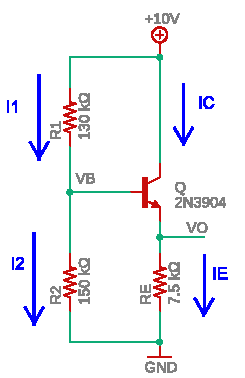
\includegraphics[width=0.4\linewidth]{./OtherFiles/Laboratorio 2/emitter follower_v2_punto di lavoro-printout}
	\caption{Analisi punto di lavoro del circuito emitter follower single-ended (seconda versione).}
	\label{fig:emitterfollwer_v2_DC}
\end{figure}

Il condensatore disaccoppia in DC i nodi ai suoi capi. Quindi viene considerato come un circuito aperto. Inoltre, si considera la corrente di base nulla. Per cui, la corrente I\sub{1} è uguale alla corrente I\sub{2}. Applicando il bilancio di correnti al nodo V\sub{B}, otteniamo la formula del partitore già mostrata (Eq.\ref{eq:1}). Per cui, considerando il transistor in regione attiva diretta, la tensione V\sub{o} sarà $V_o=V_B-\SI{0.7}{\volt}\simeq\SI{5.357}{\volt}-\SI{0.7}{\volt}=\SI{4.657}{\volt}$. Inoltre, facendo un bilancio di correnti nel transistor, si ottiene:
\begin{equation}
	\begin{split}
		I_C&=I_E \\
		&=\frac{V_o-\SI{0}{\volt}}{R_E} \\
		&=\frac{\SI{4.657}{\volt}}{\SI{7.5}{\kilo\ohm}}=\SI{0.6209}{\milli\ampere}
	\end{split}
\end{equation}






